\section{Durchführung}
\label{sec:Durchführung}

Eine Monozelle, welche aus idealer Spannungsquelle und Innenwiderstand besteht, wird
an ein Voltmeter angeschlossen, um die Leerlaufspannung der Monozelle zu  bestimmen. 
Das Voltmeter besitzt einen Widerstand von
\begin{align*}
R_\text{V} = 10\,\si{\mega\ohm}.
\end{align*}
%a)
\begin{figure}
  \centering
  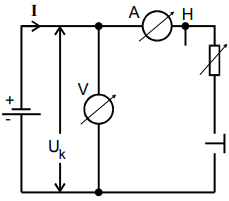
\includegraphics{schalt2.png}
  \caption{Schaltbild zur Bestimmung der Leerlaufspannung $U_\text{0}$ und 
  Innenwiderstand $R_\text{i}$. \cite[S. 3]{l} }
  \label{fig:schaltung2}
\end{figure}
Es wird ein variierbarer Belastungswiderstand (0-50\,\si{\ohm}) in Reihe geschaltet hinzugefügt.
Mit einem ebenfalls in Reihe geschalteten Amperemeter lässt sich eine Beziehung zwischen
Klemmenspannung $U_\text{K}$ und Belastungsstrom $I$ bestimmen. Das Schaltbild ist in
Abbildung 2 dargestellt. Es werden 10 Wertepaare für unterschiedliche Widerstände notiert.
%b)
\begin{figure}
  \centering
  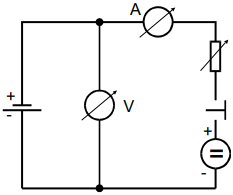
\includegraphics{schalt3.png}
  \caption{Schaltbild mit Gegenspannung. \cite[S. 3]{l} }
  \label{fig:schaltung3}
\end{figure}
Nun wird hinter den Belastungswiderstand eine Gegenspannung geschaltet, die etwa 2\,\si{\volt}
größer ist, sodass ein Strom in entgegengesetzter Richtung fließt (Abbildung 3).
Es werden erneut 10 Wertepaare von $U_\text{K}$ und $I$ notiert.
Für die letzten Messungen wird die Gegenspannung ausgebaut und die Monozelle durch einen
RC-Generator ersetzt, der zunächst eine Rechteckspannung von 1\,\si{\volt} generiert. Der Widerstand $R_\text{a}$ wird durch einen
ersetzt, der einen Variationsbereich 20-250\,\si{\ohm} aufweist. Es werden erneut die gleichen 10
Wertepaare notiert. Zuletzt wird eine Sinusspannung von 1\,\si{\volt} generiert und der Widerstand
wird durch einen mit einem Variationsbereich von 0,1\,-5\,\si{\kilo\ohm} ersetzt. Die Messung wird
erneut 10 mal durchgeführt.